\documentclass{article}

\usepackage{fancyhdr}
\usepackage{extramarks}
\usepackage{amsmath}
\usepackage{amsthm}
\usepackage{amsfonts}
\usepackage{tikz}
\usepackage[plain]{algorithm}
\usepackage{algpseudocode}
\usepackage{graphicx}
\usepackage{pgfplots}
\pgfplotsset{compat=1.18}

\usetikzlibrary{automata,positioning}

%
% Basic Document Settings
%

\topmargin=-0.45in
\evensidemargin=0in
\oddsidemargin=0in
\textwidth=6.5in
\textheight=9.0in
\headsep=0.25in

\linespread{1.1}

\pagestyle{fancy}
\lhead{Yousef Alaa Awad}
\chead{\hmwkClass\: \hmwkTitle}
\rhead{\firstxmark}
\lfoot{\lastxmark}
\cfoot{\thepage}

\renewcommand\headrulewidth{0.4pt}
\renewcommand\footrulewidth{0.4pt}

\setlength\parindent{0pt}

%
% Create Problem Sections
%

\setcounter{secnumdepth}{0}
\newcounter{partCounter}
\newcounter{homeworkProblemCounter}
\setcounter{homeworkProblemCounter}{1}

\newcommand{\hmwkTitle}{Homework\ \#2}
\newcommand{\hmwkDueDate}{February 16, 2026}
\newcommand{\hmwkClass}{Electronics 1}

%
% Title Page
%

\title{
    \vspace{2in}
    \textmd{\textbf{\hmwkClass:\ \hmwkTitle}}\\
    \normalsize\vspace{0.1in}
    \vspace{3in}
}

\author{Yousef Alaa Awad}

% \begin{figure}[!ht]
%   \centering
%   
\includegraphics[width=0.5\textwidth]{p1_42.png}
%   \caption{P1.42 from the textbook}
% \end{figure}

% Problems start here
\begin{document}

\maketitle
\pagebreak

\section{2.9}
Consider the circuits shown in Figure P2.9. Each diode cut-in voltage is $V_\gamma=0.7\ Volts$
\begin{figure}[!ht]
	\centering
	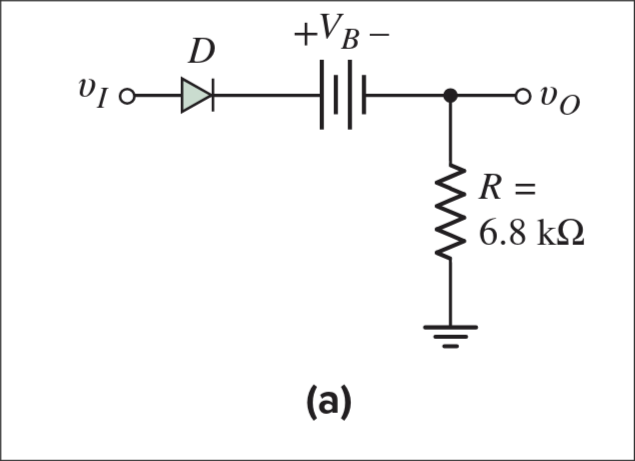
\includegraphics[width=0.5\textwidth]{p2_9.png}
	\caption{P2.9 from the textbook}
\end{figure}

\subsection{A) Plot $v_o$ versus $v_I$ over the range $-10 \le v_I \le +10$ V for the circuit in Figure P2.9(a) for...}

\subsubsection{i) $V_B = 5V$}
First we must calculate $V_I$ by doing the following:
$$ V_I - V_\gamma - V_B = V_o \rightarrow V_I = V_o + V_\gamma + V_B = 0 + 5 + 0.7 = 5.7 $$
BUT, $V_I$ is only that while it is below the cut-in voltage, meaning that while $V_I < 5.7$, $V_o = 0$.
\begin{figure}[h]
	\centering
	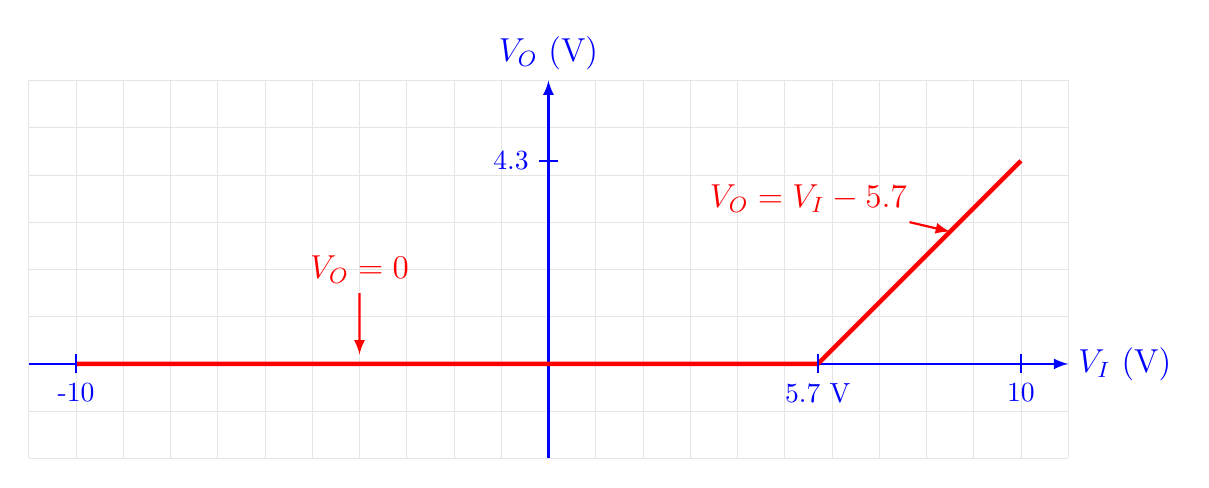
\begin{tikzpicture}[>=latex, scale=0.6]
		% 1. Draw the Grid (Optional, makes it look like graph paper)
		% defining the bounds: lower-left (-11, -2) to upper-right (11, 6)
		\draw[help lines, color=gray!20, step=1] (-11,-2) grid (11,6);

		% 2. Draw the Axes
		% X-axis
		\draw[->, thick, blue] (-11,0) -- (11,0) node[right] {\large $V_I$ (V)};
		% Y-axis
		\draw[->, thick, blue] (0,-2) -- (0,6) node[above] {\large $V_O$ (V)};

		% 3. Draw the Red Function Line
		% Part 1: Flat line from -10 to 5.7
		% Part 2: Sloped line from 5.7 to 10 (Target Y = 10 - 5.7 = 4.3)
		\draw[red, ultra thick] (-10,0) -- (5.7,0) -- (10,4.3);

		% 4. Add Ticks and Labels on Axes
		% Tick for 5.7 V
		\draw[blue, thick] (5.7, 0.2) -- (5.7, -0.2) node[blue, below] {5.7 V};
		% Tick for 4.3 on Y-axis
		\draw[blue, thick] (0.2, 4.3) -- (-0.2, 4.3) node[blue, left] {4.3};
		% Tick for -10
		\draw[blue, thick] (-10, 0.2) -- (-10, -0.2) node[blue, below] {-10};
		% Tick for 10
		\draw[blue, thick] (10, 0.2) -- (10, -0.2) node[blue, below] {10};

		% 5. Annotations (Text and Arrows)

		% "Vo = 0" with arrow
		\node[red] (lbl1) at (-4, 2) {\large $V_O = 0$};
		\draw[->, red, thick] (lbl1) -- (-4, 0.2);

		% "Vo = Vi - 5.7" with arrow
		\node[red] (lbl2) at (5.5, 3.5) {\large $V_O = V_I - 5.7$};
		\draw[->, red, thick] (lbl2) -- (8.5, 2.8);
	\end{tikzpicture}
	\caption{Transfer characteristic curve.}
\end{figure}

\pagebreak
\subsubsection{ii) $V_B = -5V$}
First we must calculate $V_I$ by doing the following:
$$ V_I - V_\gamma - V_B = V_o \rightarrow V_I = V_o + V_\gamma + V_B = 0 + 5 + (- 0.7) = 4.3 $$
BUT, $V_I$ is only that while it is below the cut-in voltage, meaning that while $V_I < -4.3$, $V_o = 0$.
\begin{figure}[h]
	\centering
	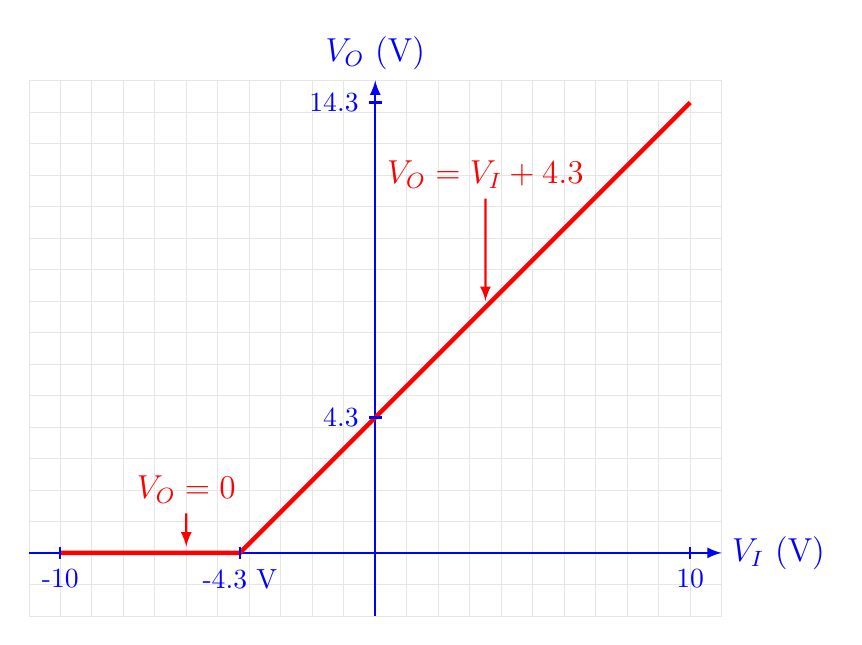
\begin{tikzpicture}[>=latex, scale=0.4]
		% 1. Draw the Grid (Optional, makes it look like graph paper)
		% defining the bounds: lower-left (-11, -2) to upper-right (11, 6)
		\draw[help lines, color=gray!20, step=1] (-11,-2) grid (11,15);

		% 2. Draw the Axes
		% X-axis
		\draw[->, thick, blue] (-11,0) -- (11,0) node[right] {\large $V_I$ (V)};
		% Y-axis
		\draw[->, thick, blue] (0,-2) -- (0,15) node[above] {\large $V_O$ (V)};

		% 3. Draw the Red Function Line
		% Part 1: Flat line from -10 to 5.7
		% Part 2: Sloped line from 5.7 to 10 (Target Y = 10 - 5.7 = 4.3)
		\draw[red, ultra thick] (-10,0) -- (-4.3,0) -- (10,14.3);

		% 4. Add Ticks and Labels on Axes
		% Tick for -4.3 V
		\draw[blue, thick] (-4.3, 0.2) -- (-4.3, -0.2) node[blue, below] {-4.3 V};
		% Tick for 4.3 on Y-axis
		\draw[blue, thick] (0.2, 4.3) -- (-0.2, 4.3) node[blue, left] {4.3};
		% Tick for 5.7 on Y-axis
		\draw[blue, thick] (0.2, 14.3) -- (-0.2, 14.3) node[blue, left] {14.3};
		% Tick for -10
		\draw[blue, thick] (-10, 0.2) -- (-10, -0.2) node[blue, below] {-10};
		% Tick for 10
		\draw[blue, thick] (10, 0.2) -- (10, -0.2) node[blue, below] {10};

		% 5. Annotations (Text and Arrows)

		% "Vo = 0" with arrow
		\node[red] (lbl1) at (-6, 2) {\large $V_O = 0$};
		\draw[->, red, thick] (lbl1) -- (-6, 0.2);

		% "Vo = Vi - 5.7" with arrow
		\node[red] (lbl2) at (3.5, 12) {\large $V_O = V_I + 4.3$};
		\draw[->, red, thick] (lbl2) -- (3.5, 8);
	\end{tikzpicture}
	\caption{Transfer characteristic curve.}
\end{figure}

\pagebreak
\subsection{B) Repeat part A for the circuit in Figure P2.9(b)}
\begin{figure}[!ht]
	\centering
	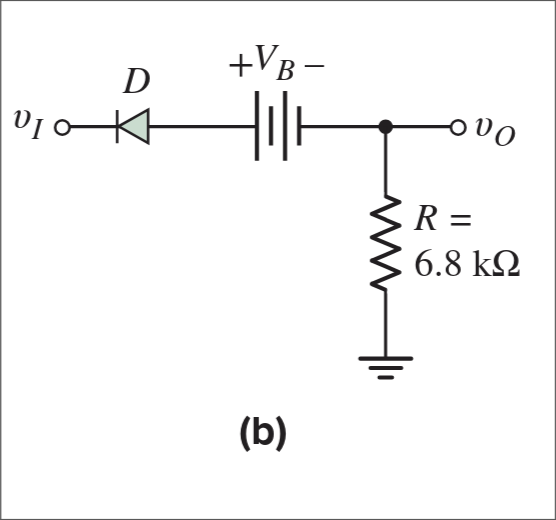
\includegraphics[width=0.5\textwidth]{p2_9b.png}
	\caption{P2.9(b) from the textbook}
\end{figure}
\subsubsection{i) $V_B = 5V$}
First we must calculate $V_I$ by doing the following:
$$ V_I - V_\gamma + V_B = V_o \rightarrow V_I = V_o + V_\gamma - V_B = 0 + 5 - 0.7 = 4.3 $$
BUT, $V_I$ is only that while it is below the cut-in voltage, meaning that while $V_I > 4.3$, $V_o = 0$.
\begin{figure}[h]
	\centering
	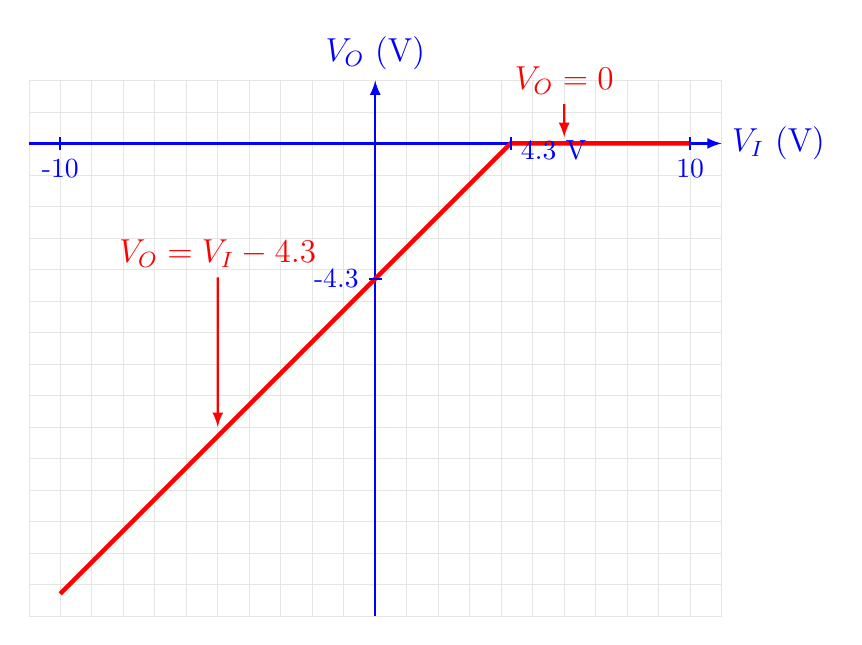
\begin{tikzpicture}[>=latex, scale=0.4]
		% 1. Draw the Grid (Optional, makes it look like graph paper)
		% defining the bounds: lower-left (-11, -2) to upper-right (11, 6)
		\draw[help lines, color=gray!20, step=1] (-11,-15) grid (11,2);

		% 2. Draw the Axes
		% X-axis
		\draw[->, thick, blue] (-11,0) -- (11,0) node[right] {\large $V_I$ (V)};
		% Y-axis
		\draw[->, thick, blue] (0,-15) -- (0,2) node[above] {\large $V_O$ (V)};

		% 3. Draw the Red Function Line
		% Part 1: Flat line from -10 to 5.7
		% Part 2: Sloped line from 5.7 to 10 (Target Y = 10 - 5.7 = 4.3)
		\draw[red, ultra thick] (-10,-14.3) -- (4.3,0) -- (10,0);

		% 4. Add Ticks and Labels on Axes
		% Tick for 5.7 V
		\draw[blue, thick] (4.3, 0.2) -- (4.3, -0.2) node[blue, right] {4.3 V};
		% Tick for 4.3 on Y-axis
		\draw[blue, thick] (0.2, -4.3) -- (-0.2, -4.3) node[blue, left] {-4.3};
		% Tick for -10
		\draw[blue, thick] (-10, 0.2) -- (-10, -0.2) node[blue, below] {-10};
		% Tick for 10
		\draw[blue, thick] (10, 0.2) -- (10, -0.2) node[blue, below] {10};

		% 5. Annotations (Text and Arrows)

		% "Vo = 0" with arrow
		\node[red] (lbl1) at (6, 2) {\large $V_O = 0$};
		\draw[->, red, thick] (lbl1) -- (6, 0.2);

		% "Vo = Vi - 5.7" with arrow
		\node[red] (lbl2) at (-5, -3.5) {\large $V_O = V_I - 4.3$};
		\draw[->, red, thick] (lbl2) -- (-5, -9);
	\end{tikzpicture}
	\caption{Transfer characteristic curve.}
\end{figure}

\pagebreak
\subsubsection{ii) $V_B = -5V$}
First we must calculate $V_I$ by doing the following:
$$ V_I - V_\gamma + V_B = V_o \rightarrow V_I = V_o + V_\gamma - V_B = 0 + 5 + 0.7 = 5.7 $$
BUT, $V_I$ is only that while it is below the cut-in voltage, meaning that while $V_I > 5.7$, $V_o = 0$.
\begin{figure}[h]
	\centering
	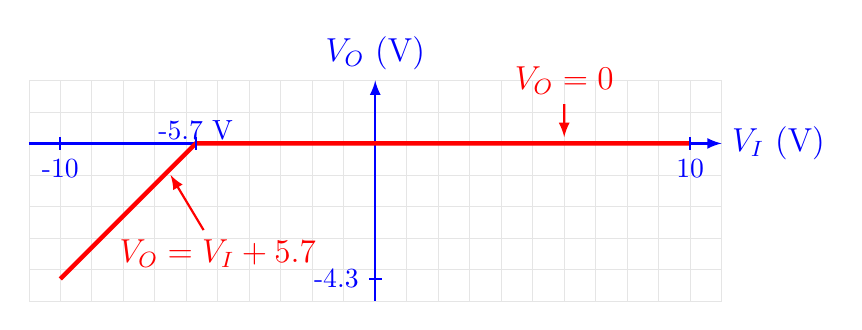
\begin{tikzpicture}[>=latex, scale=0.4]
		% 1. Draw the Grid (Optional, makes it look like graph paper)
		% defining the bounds: lower-left (-11, -2) to upper-right (11, 6)
		\draw[help lines, color=gray!20, step=1] (-11,-5) grid (11,2);

		% 2. Draw the Axes
		% X-axis
		\draw[->, thick, blue] (-11,0) -- (11,0) node[right] {\large $V_I$ (V)};
		% Y-axis
		\draw[->, thick, blue] (0,-5) -- (0,2) node[above] {\large $V_O$ (V)};

		% 3. Draw the Red Function Line
		% Part 1: Flat line from -10 to 5.7
		% Part 2: Sloped line from 5.7 to 10 (Target Y = 10 - 5.7 = 4.3)
		\draw[red, ultra thick] (-10,-4.3) -- (-5.7,0) -- (10,0);

		% 4. Add Ticks and Labels on Axes
		% Tick for 5.7 V
		\draw[blue, thick] (-5.7, 0.2) -- (-5.7, -0.2) node[blue, above] {-5.7 V};
		% Tick for 4.3 on Y-axis
		\draw[blue, thick] (0.2, -4.3) -- (-0.2, -4.3) node[blue, left] {-4.3};
		% Tick for -10
		\draw[blue, thick] (-10, 0.2) -- (-10, -0.2) node[blue, below] {-10};
		% Tick for 10
		\draw[blue, thick] (10, 0.2) -- (10, -0.2) node[blue, below] {10};

		% 5. Annotations (Text and Arrows)

		% "Vo = 0" with arrow
		\node[red] (lbl1) at (6, 2) {\large $V_O = 0$};
		\draw[->, red, thick] (lbl1) -- (6, 0.2);

		% "Vo = Vi - 5.7" with arrow
		\node[red] (lbl2) at (-5, -3.5) {\large $V_O = V_I + 5.7$};
		\draw[->, red, thick] (lbl2) -- (-6.5, -1);
	\end{tikzpicture}
	\caption{Transfer characteristic curve.}
\end{figure}

\pagebreak
\section{2.30}
Assume each diode cut-in voltage is $V_\gamma = 0.7\ Volts$ for the circuit in Figure P2.30.
\begin{figure}[!ht]
	\centering
	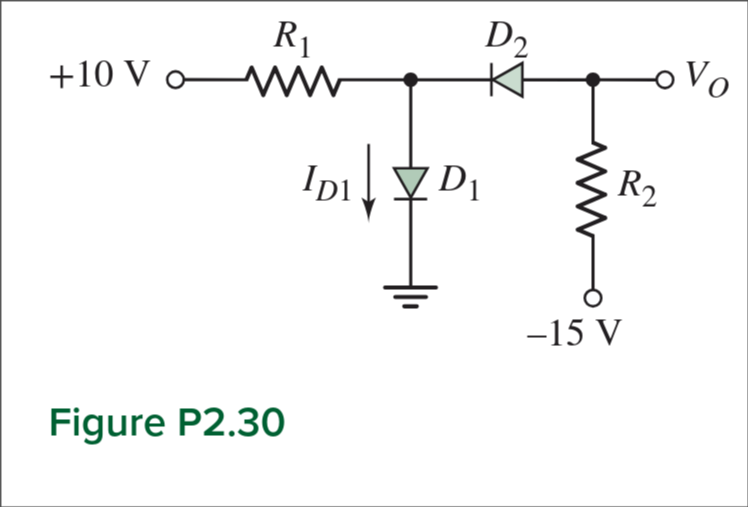
\includegraphics[width=0.5\textwidth]{p2_30.png}
	\caption{P2.30 from the textbook}
\end{figure}

\subsection{A) Determine $I_{D1}$ and $V_O$ for $R_1 = 10k \Omega $, $R_2 = 5k \Omega $}
We can derive the following equation from the circuit...
$$ 10 - I_1*R_1 - V_{D1} = 0 $$
Now, assuming that $I_1 = 0$, $V_{D1} = 10$, this means that $Diode_1$ is on and $Diode_2$ is off, therefore...
$$ 10 - I_1*R_1 - 0.7 = 0 \rightarrow I_{D1} = I_1 \frac{9.3}{10,000} = 0.93mA $$
This then means that the $V_o$ is going to simply be the same voltage as the load since diode 2 is off... Therefore...
$$ V_o = -15\ V $$

\subsection{B) Determine $I_{D1}$ and $V_O$ for $R_1 = 5k \Omega $, $R_2 = 10k \Omega $}
Now, since the circuit is unchanged, we can assume that $I_1 = 0$, $V_{D1} = 10$, this, again, means that $Diode_1$ is on and $Diode_2$ is off, therefore...
$$ 10 - I_1*R_1 - 0.7 = 0 \rightarrow I_{D1} = I_1 \frac{10 - 0.7}{5,000} = 1.86mA $$
This then means that the $V_o$ is going to simply be the same voltage as the load since diode 2 is off... Therefore...
$$ V_o = -15\ V $$


\pagebreak
\section{2.40}
For the circuit shown in Figure P2.39, show that for $v_1 \ge 0$, the output voltage is approximately given by...
$$ v_o = v_I - V_T*ln(\frac{v_o}{I_S*R}) $$
\begin{figure}[!ht]
	\centering
	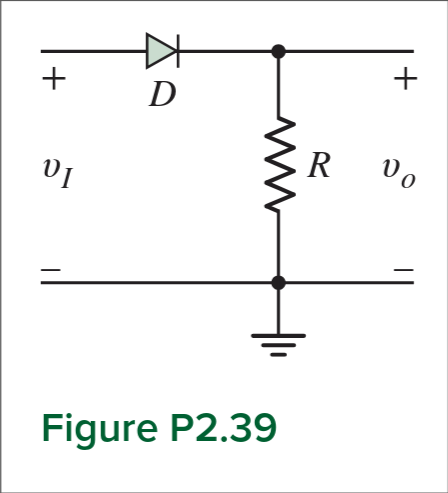
\includegraphics[width=0.5\textwidth]{p2_39.png}
	\caption{P2.39 from the textbook}
\end{figure}

\subsection{Proof}
Given the following 2 equations:
$$ I_D = I_S*(e^{\frac{V_D}{n*V_T}} - 1) $$
$$ V_I = V_D + V_o \rightarrow V_o = V_I - V_o $$
We can do the following...
$$ V_O = I_D*R == I_S*(e^{\frac{V_D}{n*V_T}} - 1)*R \rightarrow \frac{V_o}{I_S*R} = e^{\frac{V_I - V_o}{n*V_T}} - 1 \rightarrow$$
$$ \frac{V_I - V_o}{n*V_T} = ln(\frac{V_o}{I_S*R} + 1) $$
And, when we rearrange the equation to solve for $V_o$, we get...
$$ V_o = V_I - n*V_T*ln(\frac{V_o}{I_S*R} + 1) \approx V_I - V_T*ln(\frac{V_o}{I_s*R}) $$

\pagebreak
\section{2.52}
The circuit in Figure P2.52 is a complementary output rectifier. If $v_s = 26*sin[2*\pi*(60\ Hz)*t]$ Volts, sketch the output waveforms $v_o^+$ and $v_o^-$ versus time, assuming $V_\gamma = 0.6\ V$ for each diode.
\begin{figure}[!ht]
	\centering
	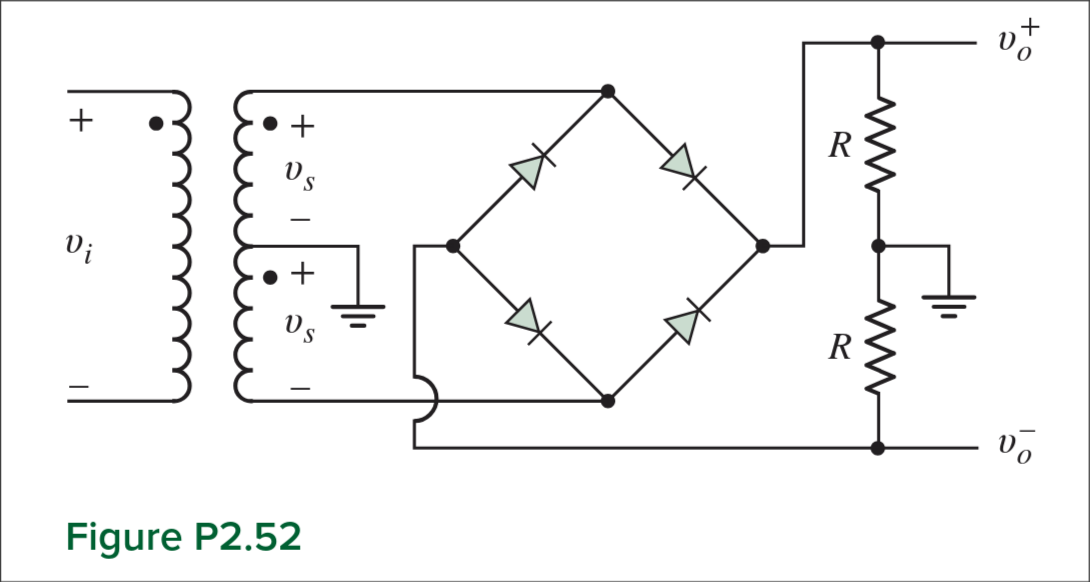
\includegraphics[width=0.5\textwidth]{p2_52.png}
	\caption{P2.52 from the textbook}
\end{figure}

The following is the waveform

\begin{center}
	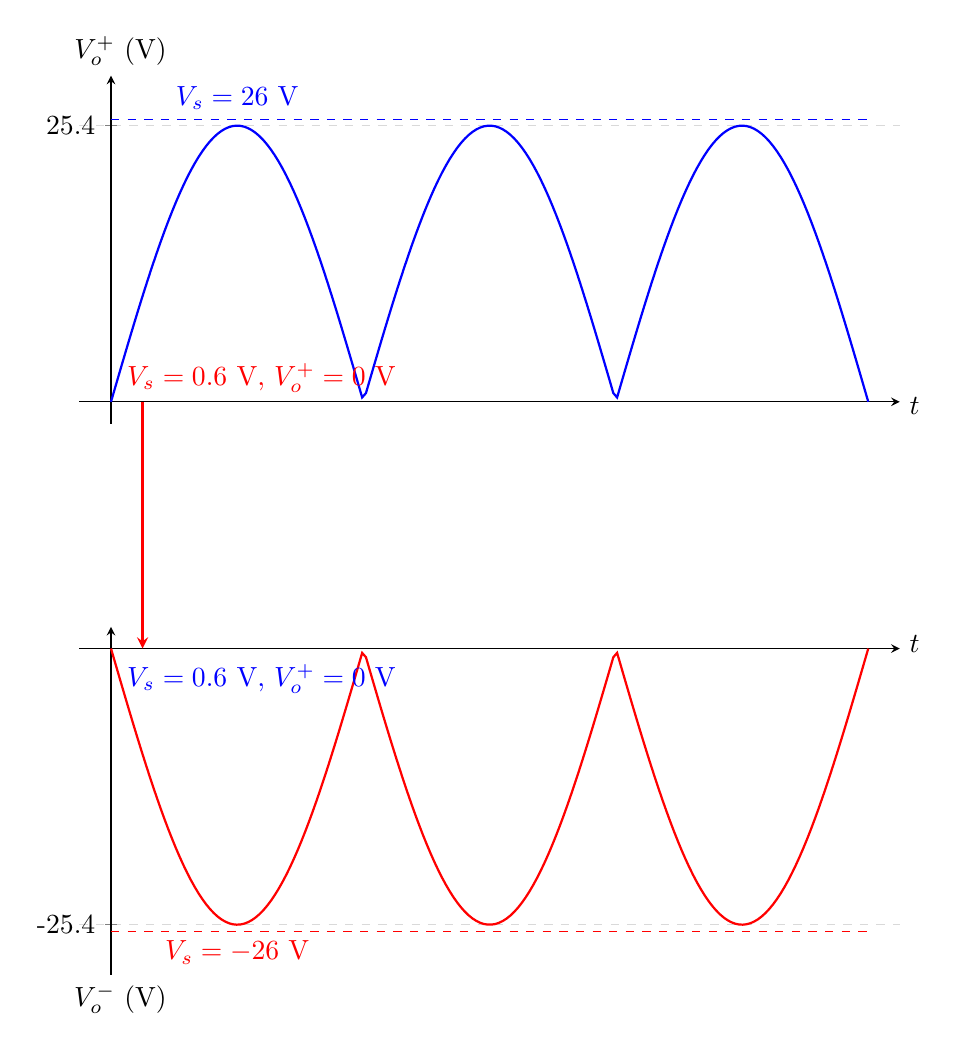
\begin{tikzpicture}
		% Top Graph: Vo+ (V)
		\begin{axis}[
				width=12cm, height=6cm,
				axis lines=middle,
				xlabel={$t$}, ylabel={$V_o^+$ (V)},
				xmin=-0.5, xmax=12.5,
				ymin=-2, ymax=30,
				xtick={\empty},
				ytick={0, 25.4},
				yticklabels={0, 25.4},
				grid=major,
				grid style={dashed, gray!30},
				ylabel style={at={(axis description cs:0.05,1)},anchor=south},
				xlabel style={at={(axis description cs:1,0.05)},anchor=west},
			]
			% Plot Vo+ curve (rectified sine)
			\addplot[blue, thick, samples=200, domain=0:12] {25.4 * abs(sin(deg(x*pi/4)))};

			% Dashed line for peak voltage
			\draw[blue, dashed] (axis cs:0,26) -- (axis cs:12,26);
			\node[blue, anchor=south] at (axis cs:2, 26) {$V_s=26$ V};

			% Annotation at t=0
			\node[red, anchor=south west] at (axis cs:0.1, 0) {$V_s=0.6$ V, $V_o^+=0$ V};

			% Coordinate for arrow start
			\coordinate (arrow_start) at (axis cs:0.5, 0);
		\end{axis}

		% Bottom Graph: Vo- (V)
		\begin{axis}[
				width=12cm, height=6cm,
				at={(0,-7cm)}, % Position below the top graph
				axis lines=middle,
				xlabel={$t$}, ylabel={$V_o^-$ (V)},
				xmin=-0.5, xmax=12.5,
				ymin=-30, ymax=2,
				xtick={\empty},
				ytick={0, -25.4},
				yticklabels={0, -25.4},
				grid=major,
				grid style={dashed, gray!30},
				ylabel style={at={(axis description cs:0.05,0)},anchor=north},
				xlabel style={at={(axis description cs:1,0.95)},anchor=west},
			]
			% Plot Vo- curve (negative rectified sine)
			\addplot[red, thick, samples=200, domain=0:12] {-25.4 * abs(sin(deg(x*pi/4)))};

			% Dashed line for trough voltage
			\draw[red, dashed] (axis cs:0,-26) -- (axis cs:12,-26);
			\node[red, anchor=north] at (axis cs:2, -26) {$V_s=-26$ V};
			\node[blue, anchor=south west] at (axis cs:0.1, -5) {$V_s=0.6$ V, $V_o^+=0$ V};

			% Coordinate for arrow end
			\coordinate (arrow_end) at (axis cs:0.5, 0);
		\end{axis}

		% Red connecting arrow
		\draw[red, thick, ->, >=stealth, out=270, in=90] (arrow_start) to (arrow_end);

	\end{tikzpicture}
\end{center}

\pagebreak
\section{2.59}
Consider the Zener diode circuit shown in Figure P2.59. Let $V_I = 60 V$, $R_i = 150\Omega$, and $V_{ZO} = 15.4 V$. Assume $r_z = 0$. The power rating of the diode is 4W and the minimum diode current is to be 15mA.
\begin{figure}[!ht]
	\centering
	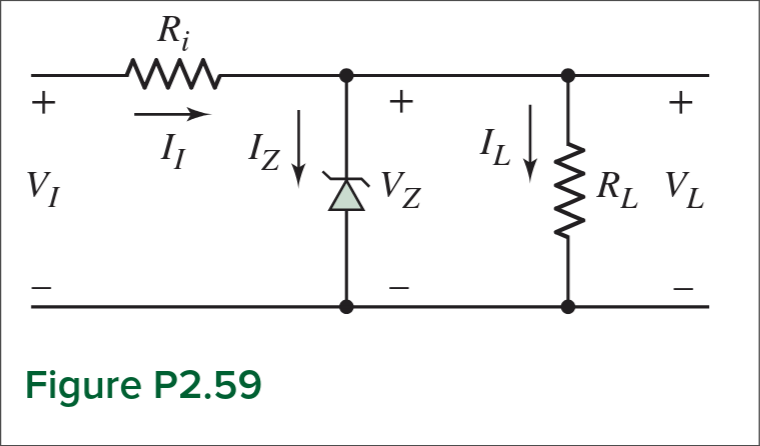
\includegraphics[width=0.5\textwidth]{p2_59.png}
	\caption{P2.59 from the textbook}
\end{figure}

\subsection{A) Determine the range of diode currents.}
$$ I_{(2,\ max)} = \frac{P_{(2, max)}}{V_ZO} = \frac{4mW}{15.4V} = 259.74mA $$
Therefore the range is...
$$ 15mA \le I_Z \le 259.74mA $$

\subsection{B) Determine the range of load resistance.}
Now...
$$ V_I - I_I*R_i - V_Z = 0 \rightarrow I_I = \frac{V_I - V_Z}{R_i} = \frac{60 - 15.4}{150} = 297.33mA $$
And then...
$$ I_L = I_I - I_Z = either... $$
With the minimum current:
$$ I_L = I_I - I_{(Z,\ max)} = 297.33 - 259.74 = 37.59mA $$
$$ I_L = I_I - I_{(Z,\ min)} = 297.33 - 15 = 282.33mA $$
and therefore using Ohm's Law we get a load restance range of...
$$ \frac{V_Z}{I_{(L, max)}} \le R_L \le \frac{V_Z}{I_{(L, min)}} \rightarrow 54.545 \Omega \le R_L \le 409.650 \Omega $$


\end{document}

